\chapter{Cluster analysis}


Finding groups of objects such that the objects in a group
will be similar (or related) to one another and different
from (or unrelated to) the objects in other groups.

The aim of clustering is to ease data \textbf{understanding} and \textbf{summarization}, i.e. reduce the size of data sets.

\note{
	The following are \textit{NOT} cluster analysis:
	\begin{itemize}
		\item Simple segmentation
		\begin{itemize}
			\item Dividing students into different registration groups
		\end{itemize}
		alphabetically, by last name
		\item Results of a query
		      \begin{itemize}
			      \item Groupings are a result of an external specification
			      \item Clustering is a grouping of objects based on the data
		      \end{itemize}
		\item Supervised classification
		      \begin{itemize}
			      \item Have class label information
		      \end{itemize}
		\item Association Analysis
		      \begin{itemize}
			      \item Local vs. global connections
		      \end{itemize}
	\end{itemize}

	These ain't clustering essentially because there is no \textbf{similarity} measure involved, which instead is the core of clustering.
}

\begin{figure}[htbp]
   \centering
   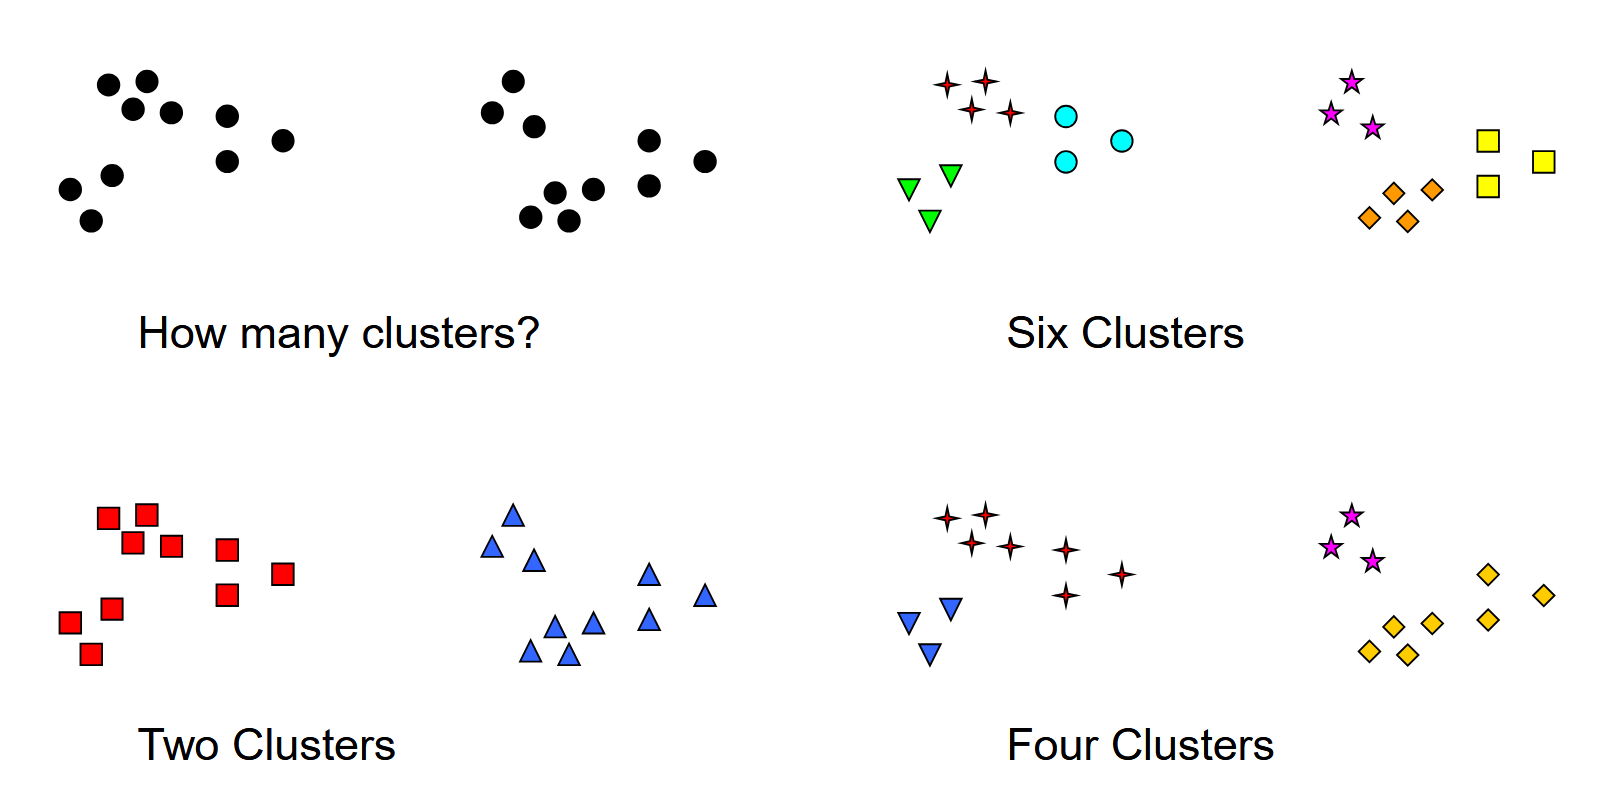
\includegraphics{images/04/clustering.png}
   \caption{``Cluster'' may be an amibguous term. How to define a cluster? How big is a cluster? How many clusters are there?}
   \label{fig:04/clustering}
\end{figure}

\section{Definitions}
A \textbf{clustering} is a set of clusters. There is an important distinction between hierarchical and
partitional sets of clusters.
\begin{itemize}
	\item \textit{Partitional} Clustering\\
	A division of data objects into non-overlapping subsets
	(clusters) such that each data object is in exactly one subset.
	\item \textit{Hierarchical} Clustering\\
	A set of nested clusters organized as a hierarchical tree.
\end{itemize}

\begin{figure}[htbp]
	\centering
	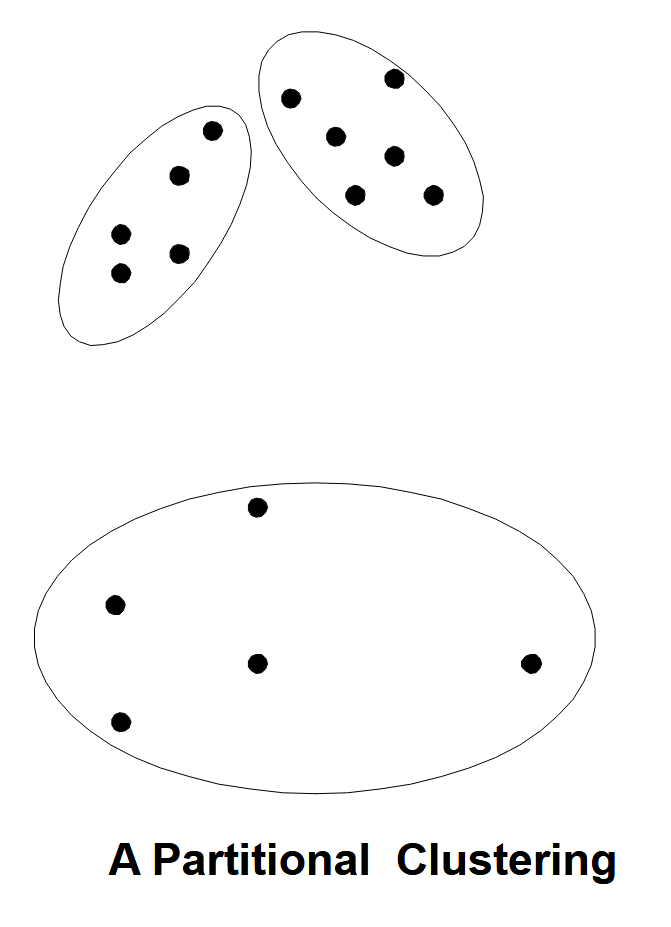
\includegraphics[width=0.33\columnwidth]{images/04/partitional.png}
	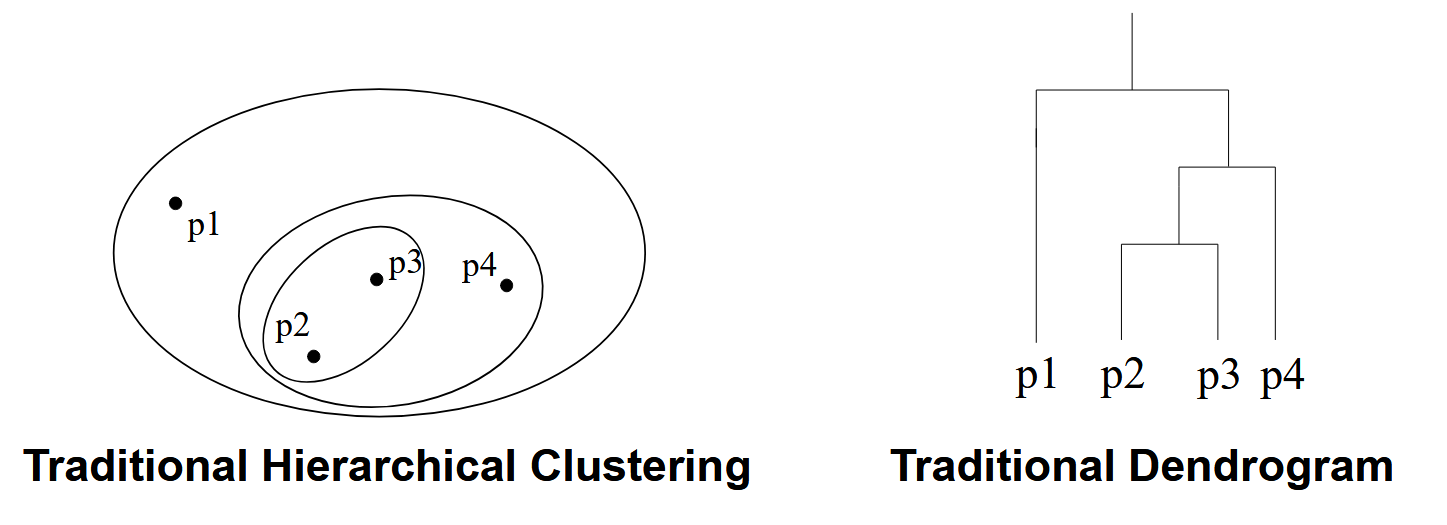
\includegraphics[width=0.66\columnwidth]{images/04/hierarchical.png}
	\caption{Partitional vs Hierarchical clustering}
	\label{fig:04/partitional_hierarchical}
\end{figure}


There are other distinctions among clusterings:
\begin{itemize}
	\item Exclusive versus non-exclusive
	      \begin{itemize}
		      \item In non-exclusive clusterings, points may belong to multiple
	      \end{itemize}
	      clusters.
	      \begin{itemize}
		      \item Can represent multiple classes or ‘border’ points
	      \end{itemize}
	\item Fuzzy versus non-fuzzy
	      \begin{itemize}
		      \item In fuzzy clustering, a point belongs to every cluster with some
		            weight between 0 and 1
		      \item Weights must sum to 1
		      \item Probabilistic clustering has similar characteristics
	      \end{itemize}
	\item Partial versus complete
	      \begin{itemize}
		      \item In some cases, we only want to cluster some of the data
	      \end{itemize}
	\item Heterogeneous versus homogeneous
	      \begin{itemize}
		      \item Clusters of widely different sizes, shapes, and densities
	      \end{itemize}
\end{itemize}

\section{Types of Clustering}
% // TODO add pictures
\begin{itemize}
	\item Well-separated clusters
	      A cluster is a set of points such that any point in a cluster is closer (or more similar) to every other point in the cluster than to any point not in the cluster
	\item Center-based clusters
	      \begin{paracol}{2}
		      \begin{figure}[htbp]
			      \centering
			      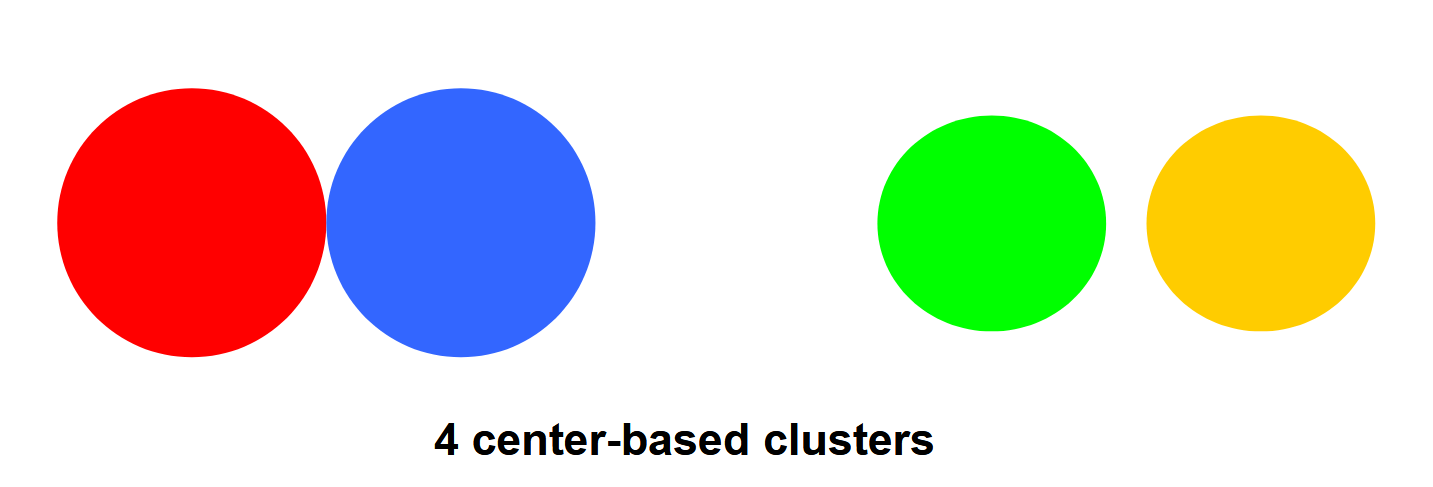
\includegraphics{images/04/centerbased.png}
			      \caption{Center-based clusters}
			      \label{fig:04/centerbased}
		      \end{figure}
		      \switchcolumn

		      \begin{itemize}
			      \item A cluster is a set of objects such that an object in a cluster is
			            closer (more similar) to the “center” of a cluster, than to the
			            center of any other cluster
			      \item The center of a cluster is often a centroid, the average of all
			            the points in the cluster, or a medoid, the most “representative”
			            point of a cluster
		      \end{itemize}
	      \end{paracol}
	\item Contiguous clusters (Nearest neighbor or
	      Transitive)

	      \begin{paracol}{2}
		      \colfill
		      \begin{itemize}
			      \item Each point is closer to at least one point in its cluster than to
			            any point in another cluster.
			      \item Graph based clustering
			      \item This approach can have trouble when noise is present since a
			            small bridge of points can merge two distinct clusters
		      \end{itemize}

		      \colfill
		      \switchcolumn

		      \begin{figure}[htbp]
			      \centering
			      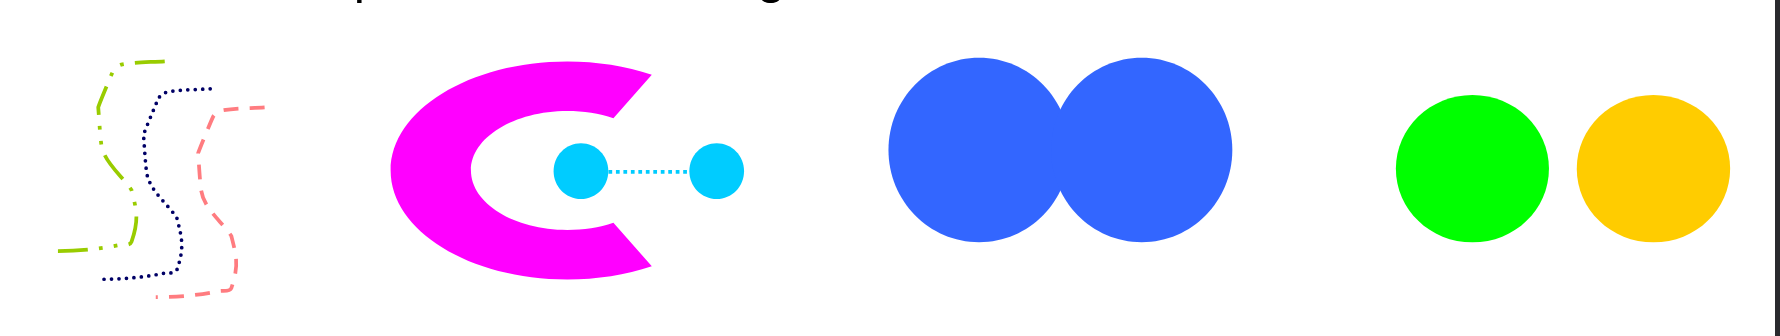
\includegraphics{images/04/contiguitybased.png}
			      \caption{Contiguity-based clusters}
			      \label{fig:04/contiguitybased}
		      \end{figure}

	      \end{paracol}

	\item Density-based clusters
	      \begin{paracol}{2}
		      \colfill
		      \begin{itemize}
			      \item A cluster is a dense region of points, which is separated by
			            low-density regions, from other regions of high density.
			      \item Used when the clusters are irregular or intertwined, and when
			            noise and outliers are present.
			      \item Points which are not classfied as part of any cluster are considered noise. In the figure they may be the gray blackground points.
		      \end{itemize}
		      \colfill
		      \switchcolumn
		      \begin{figure}[htbp]
			      \centering
			      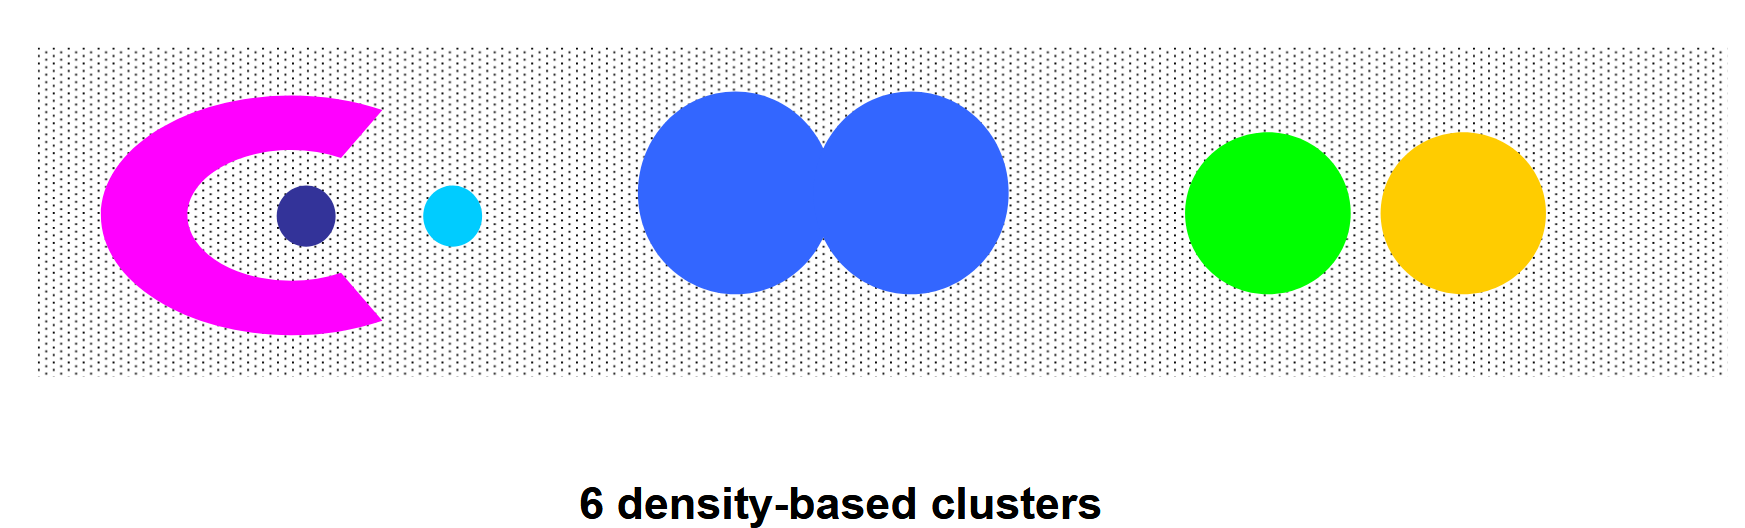
\includegraphics{images/04/densitybased.png}
			      \caption{Density-based clusters}
			      \label{fig:04/densitybased}
		      \end{figure}
	      \end{paracol}
	\item Property or Conceptual
	\item Described by an Objective Function
	      \begin{itemize}
		      \item Finds clusters that minimize or maximize an objective
		            function.
		      \item Enumerate all possible ways of dividing the points into
		            clusters and evaluate the `goodness' of each potential
		            set of clusters by using the given objective function.
		      \item NP Hard)
		      \item Can have global or local objectives.
		            \begin{itemize}
			            \item Hierarchical clustering algorithms typically have local objectives
			            \item Partitional algorithms typically have global objectives
		            \end{itemize}
	      \end{itemize}
\end{itemize}

\newpage
\section{Similarity}
\begin{itemize}
    \item Similarity
          \begin{itemize}
              \item Numerical measure of how alike two data objects are.
              \item Is higher when objects are more alike.
              \item Often falls in the range [0,1]
          \end{itemize}
    \item Dissimilarity
          \begin{itemize}
              \item Numerical measure of how different are two data objects
              \item Lower when objects are more alike
              \item Minimum dissimilarity is often 0
              \item Upper limit varies
          \end{itemize}
    \item Proximity refers to a similarity or dissimilarity
\end{itemize}

\subsection{Similarity and Dissimilarity for Different Attribute Types}

\begin{table}[htbp]
\centering
\caption{Similarity and dissimilarity for simple attributes}
\begin{tabular}{|p{3cm}|p{6cm}|p{4cm}|}
\hline
\textbf{Attribute Type} & \textbf{Dissimilarity} & \textbf{Similarity} \\
\hline
Nominal & 
$d = \begin{cases}
0 & \text{if } p = q \\
1 & \text{if } p \neq q
\end{cases}$ & 
$s = \begin{cases}
1 & \text{if } p = q \\
0 & \text{if } p \neq q
\end{cases}$ \\
\hline
Ordinal & 
$d = \frac{|p-q|}{n-1}$

(values mapped to integers 0 to $n-1$, where $n$ is the number of values) & 
$s = 1 - \frac{|p-q|}{n-1}$ \\
\hline
Interval or Ratio & 
$d = |p - q|$ & 
$s = -d$, $s = \frac{1}{1+d}$ or

$s = 1 - \frac{d-min\_d}{max\_d-min\_d}$ \\
\hline
\end{tabular}
\label{tab:similarity_attributes}
\end{table}

$p$ and $q$ are the attribute values for two data objects.

\subsection{Euclidean Distance}
The most common way to measure distance between two data objects is the Euclidean distance:

\[
d(\mathbf{x}, \mathbf{y}) = \sqrt{\sum_{k=1}^{n}(x_k - y_k)^2}
\]

where $n$ is the number of dimensions (attributes) and $x_k$ and $y_k$ are, respectively, the $k^{th}$ attributes (components) or data objects $\mathbf{x}$ and $\mathbf{y}$. Standardization is necessary, if scales differ.

\begin{itemize}
    \item Standardization is necessary, if scales differ.
\end{itemize}


\subsubsection{Minkowski Distance}

Minkowski Distance is a generalization of Euclidean Distance. $r$ is a parameter that defines the type of distance, $n$ is the number of dimensions (attributes) and $x_k$ and $y_k$ are, respectively, the $k^{th}$ attributes (components) or data objects $\mathbf{x}$ and $\mathbf{y}$.

\[
d(\mathbf{x}, \mathbf{y}) = \left(\sum_{k=1}^{n} |x_k - y_k|^r\right)^{\frac{1}{r}}
\]

\begin{itemize}
	\item For $r=1$, it is the Manhattan distance (or city block/Hamming distance)
	\item For $r=2$, it is the Euclidean distance
	\item For $r \rightarrow \infty$, it is the supremum distance (or Chebyshev distance)
\end{itemize}

\framedt{Metrics and Similiraties}{
	\begin{enumerate}
		\item $d(x, y) \geq 0$ for all $x$ and $y$ and $d(x, y) = 0$ only if
		      $x = y$. (Positive definiteness)
		\item $d(x, y) = d(y, x)$ for all $x$ and $y$. (Symmetry)
		\item $d(x, z) \leq d(x, y) + d(y, z)$ for all points $x$, $y$, and $z$ (Triangle Inequality).
	\end{enumerate}
	A \textit{distance} $d$ is a \textit{metric} if it satisfies the three conditions above.

	\begin{enumerate}
			\item $s(x, y) = 1$ (or maximum similarity) only if $x = y$.
			\item $s(x, y) = s(y, x)$ for all $x$ and $y$. (Symmetry)
	\end{enumerate}
	These instead are properties of a \textit{similarity} measure.
}

\subsection{Binary Similarity}
Computing similarity among objects described by binary attributes is slightly different from numerical attributes.
\begin{itemize}
	\item Simple Matching Coefficient (SMC)
	      \[
		      SMC = \frac{\texttt{\#matches}}{\texttt{\#attributes}}=\frac{f_{11} + f_{00}}{f_{11} + f_{10} + f_{01} + f_{00}}
	      \]
	\item Jaccard Coefficient
	      \[
		      J = \frac{\texttt{\#}11\texttt{matches}}{\texttt{\#non-zero attribute values}}\frac{f_{11}}{f_{11} + f_{10} + f_{01}}
	      \]
\end{itemize}

\begin{align*}
	p &= 1\ 0\ 0\ 0\ 0\ 0\ 0\ 0\ 0\ 0\\
	q &= 0\ 0\ 0\ 0\ 0\ 0\ 1\ 0\ 0\ 1\\
	f_{01} &= 2 \text{ (\#attributes where } p \text{ was 0 and } q \text{ was 1)}\\
	f_{10} &= 1 \text{ (\#attributes where } p \text{ was 1 and } q \text{ was 0)}\\
	f_{00} &= 7 \text{ (\#attributes where } p \text{ was 0 and } q \text{ was 0)}\\
	f_{11} &= 0 \text{ (\#attributes where } p \text{ was 1 and } q \text{ was 1)}\\
	SMC &= \frac{0 + 7}{10} = 0.7\\
	J &= \frac{0}{0 + 1 + 2} = 0
\end{align*}

\subsection{Cosine Similarity}
Used often in text mining, where each dimension corresponds to a term (word) and the value
of the dimension is the frequency of the term in the document.

If $d_1$ and $d_2$ are two document vectors, then
\[
	\cos( d_1, d_2 ) = (d_1 \cdot d_2) / ||d_1|| ||d_2||
\]
where $\cdot$ indicates vector dot product and $||d||$ is the length of vector $d$.

Example:
\begin{align*}
	d_1 &= 3\ 2\ 0\ 5\ 0\ 0\ 0\ 2\ 0\ 0\\
	d_2 &= 1\ 0\ 0\ 0\ 0\ 0\ 0\ 1\ 0\ 2\\
	d_1 \cdot d_2 &= 3*1 + 2*0 + 0*0 + 5*0 + 0*0 + 0*0 + 0*0 + 2*1 + 0*0 + 0*2 = 5\\
	||d_1|| &= \sqrt{3^2 + 2^2 + 0^2 + 5^2 + 0^2 + 0^2 + 0^2 + 2^2 + 0^2 + 0^2} = \sqrt{42}\\
	||d_2|| &= \sqrt{1^2 + 0^2 + 0^2 + 0^2 + 0^2 + 0^2 + 0^2 + 1^2 + 0^2 + 2^2} = \sqrt{6}\\
	\cos(d_1, d_2) &= \frac{5}{\sqrt{42} * \sqrt{6}} = \frac{5}{\sqrt{252}} \approx 0.315
\end{align*}


\subsection{Correlation}

\begin{paracol}{2}
	
	\begin{figure}[htbp]
		\centering
		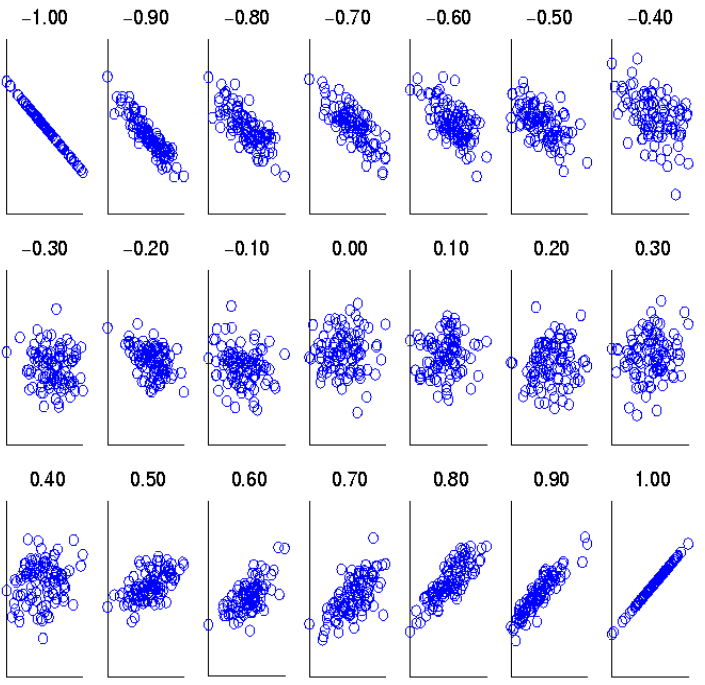
\includegraphics{images/04/correlation.png}
		\caption{Scatter plots showing the similarity from -1 to 1}
		\label{fig:04/correlation}
	\end{figure}
	\switchcolumn
	\colfill
	Correlation measures the linear relationship between objects (binary or continuous).
	To compute correlation, we standardize data objects, $p$ and $q$, and then take their dot product (covariance/standard deviation).
	\colfill
\end{paracol}
	\[
		corr(\mathbf{x},\mathbf{y}) = \frac{covariance(\mathbf{x},\mathbf{y})}{stddev(\mathbf{x})*stddev(\mathbf{y})} = \frac{\sum_{k=1}^{n}(x_k - \bar{x})(y_k - \bar{y})}{\sqrt{\sum_{k=1}^{n}(x_k - \bar{x})^2}\sqrt{\sum_{k=1}^{n}(y_k - \bar{y})^2}}
		\]
		

\subsection{Entropy}
Information relates to possible outcomes of an event such as transmission of a message, flip of a coin, or measurement of a piece of data.
\ul{The amount of information is inversely related to the probability of an event}.
Entropy is the commonly used measure of information content.
For a discrete random variable $X$ with $n$ possible values ${x_1, x_2, ..., x_n}$ each having probability $p_1,p_2,\dots,p_n$, the entropy $H(X)$ is defined as:
\[
H(X) = -\sum_{i=1}^{n} p_i \log_2(p_i)
\]

Entropy is measured in bits and is $0 \leq H(X) \leq \log_2(n)$. Thus, entropy is a measure of how many bits it takes to represent an observation of $X$ on average.

The information one variable provides about another is called mutual information.
The mutual information $I(X;Y)$ of two discrete random variables $X$ and $Y$ is defined as:
\[
I(X,Y) = H(X) + H(Y) - H(X,Y) = \sum_{x \in X} \sum_{y \in Y} p(x,y) \log_2p(x,y)
\]
where $H(X,Y)$ is the joint entropy of $X$ and $Y$, and $p(x,y)$ is the probability that $x$ and $y$ occur together.

\section{K-Means}
\begin{itemize}
	\item \textit{Partitional} clustering approach
	\item The number of clusters $K$, must be specified
	\item Each cluster is associated with a \textbf{centroid} (center point), typically being the mean of the points in the cluster
	\item Each point is assigned to the cluster with the closest centroid. This may measured as Euclidean distance, cosine similarity, correlation, etc.
	\note{Using these measures makes K-Means to converge in the first few iterations.}
	\item Complexity is $O(nKId)$, where $n$ is the number of data points, $K$ is the number of clusters, $I$ is the number of iterations, and $d$ is the number of dimensions (attributes)
	\item The basic algorithm is very simple
\end{itemize}

\begin{algorithm}[H]
\caption{K-Means Clustering Algorithm}
\begin{algorithmic}[1]
\State Select $K$ points as the initial centroids.
\Repeat
\State Form $K$ clusters by assigning all points to the closest centroid.
\State Recompute the centroid of each cluster.
\Until{The centroids don't change}
\end{algorithmic}
\end{algorithm}

\begin{figure}[htbp]
	\centering
	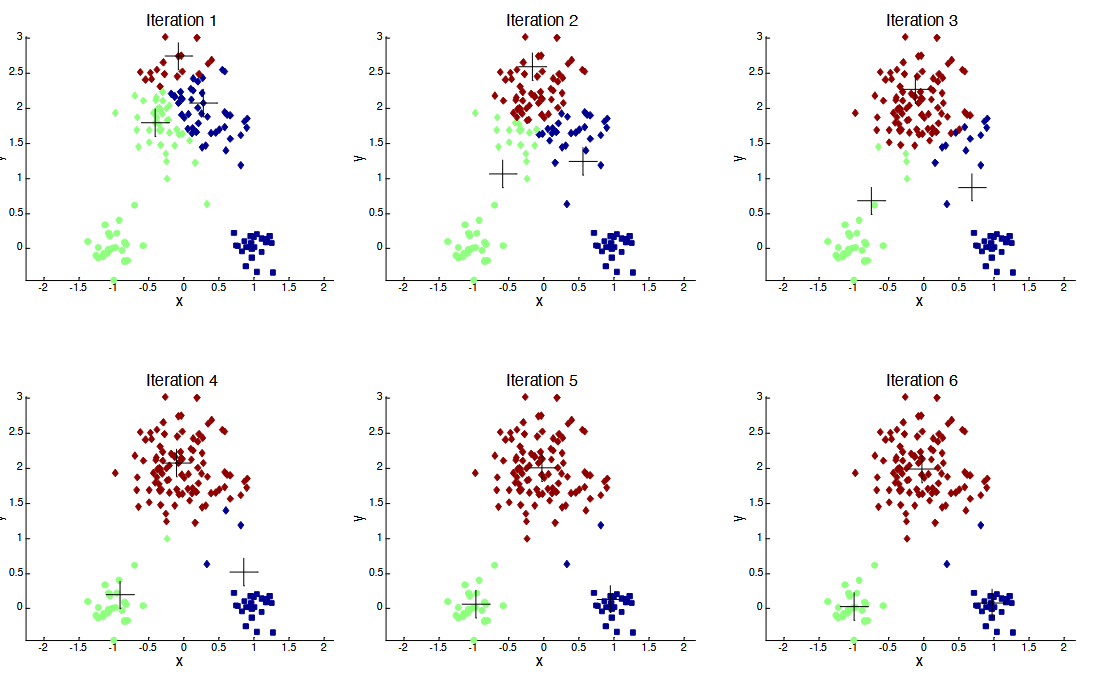
\includegraphics{images/04/kmeans.png}
	\caption{K-Means Clustering Iterations}
	\label{fig:kmeans}
\end{figure}

\subsection{Evaluating K-Means clusters}
The most common measure to evaluate the quality of K-Means clusters is the \textbf{Sum of Squared Errors} (SSE), also known as \textbf{Inertia}. It quantifies how tightly the data points in a cluster are grouped around their centroid. The SSE is calculated as follows:
\[
SSE = \sum_{i=1}^{K} \sum_{x \in C_i} ||x - \mu_i||^2
\]
\note{
	\begin{itemize}
	\item $K$ is the number of clusters,
	\item $C_i$ is the set of points in cluster $i$,
	\item $x$ is a data point in cluster $C_i$,
	\item $\mu_i$ is the centroid of cluster $C_i$,
	\item $||x - \mu_i||^2$ is the squared Euclidean distance between point $x$ and centroid $\mu_i$.
\end{itemize}
}

\subsection{Limitations of K-Means}

\begin{paracol}{2}
	\colfill
	K-means has problems when clusters are of differing
	\begin{itemize}
		\item Clusters have different sizes
		\item Clusters have different densities
		\item Clusters have Non-globular shapes
		\item The data contains \textbf{outliers}.
	\end{itemize}
	\colfill
	\switchcolumn
	\begin{figure}[htbp]
		\centering
		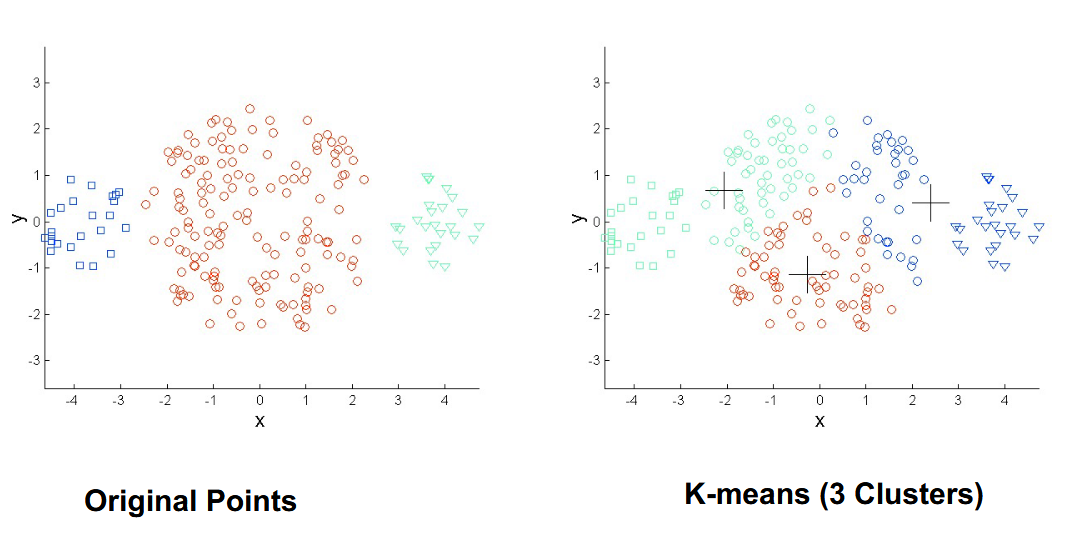
\includegraphics[width=0.9\columnwidth]{images/04/kproblems.png}
		\caption{K-Means with different cluster sizes}
		A solution may be to use more clusters, hence increasing $K$, and then merging them.
		\label{fig:04/kproblems}
	\end{figure}

\end{paracol}

\begin{figure}[htbp]
	\centering
	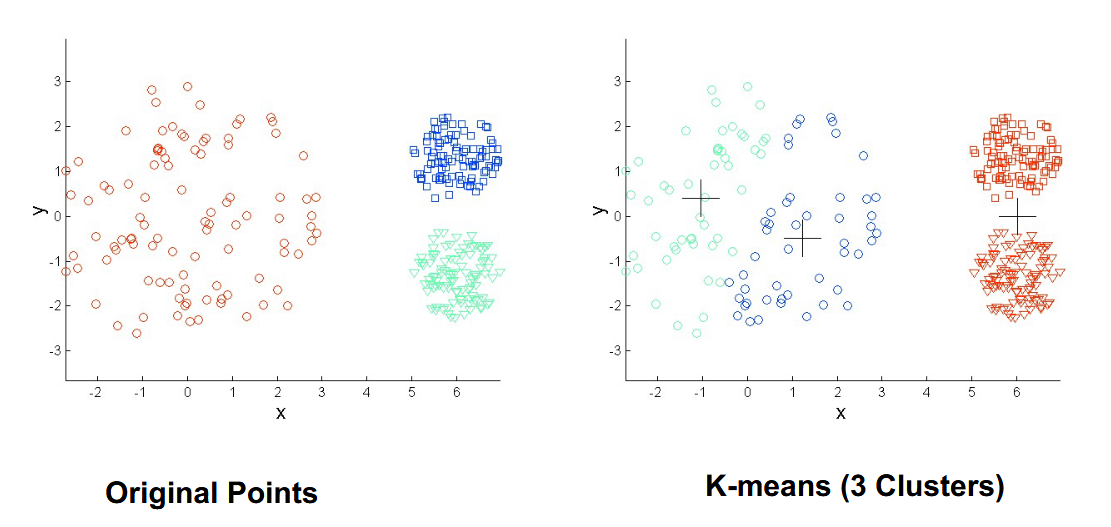
\includegraphics[width=0.48\columnwidth]{images/04/kdensity.png}
	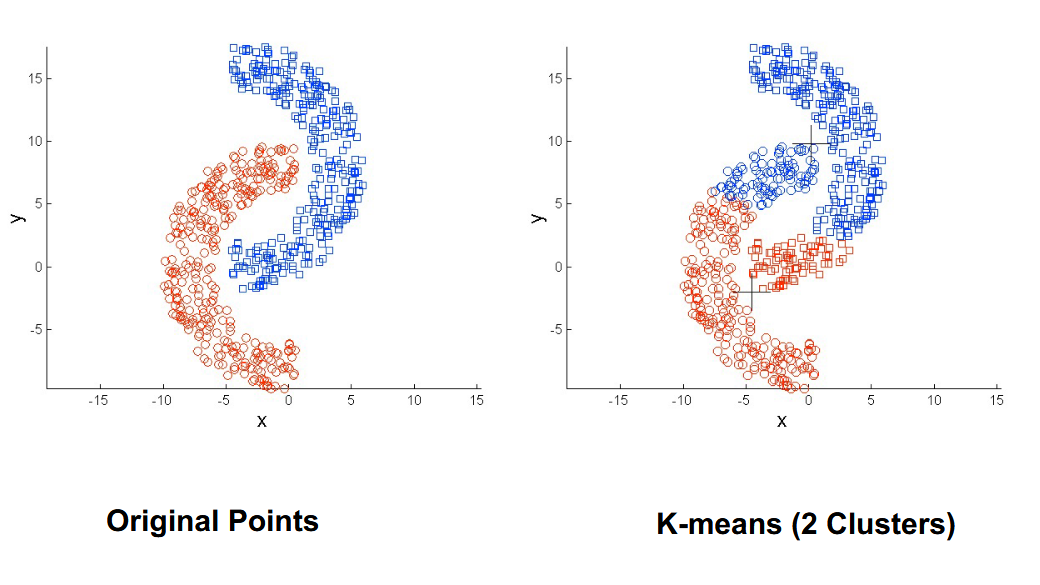
\includegraphics[width=0.48\columnwidth]{images/04/kglobular.png}
	\caption{K-Means with different cluster densities and non-globular shapes}
	\label{fig:04/kdensity}
\end{figure}

\subsubsection{Empty Clusters}

\begin{paracol}{2}
	
	K-Means sometimes produces empty clusters. This happens when no points are assigned to a cluster during the assignment step. This can occur if the initial centroids are poorly chosen or if the data distribution is such that certain centroids end up being too far from any data points.

	 Solutions include the following strategies, which may be iterated until no empty clusters remain:
	\begin{itemize}
		\item Choose a point and assign it to the cluster
		\begin{itemize}
			\item Choose the point that contributes most to SSE
			\item Choose a point from the cluster with the highest SSE
		\end{itemize}
	\end{itemize}

	\switchcolumn

	\begin{figure}[htbp]
		\centering
		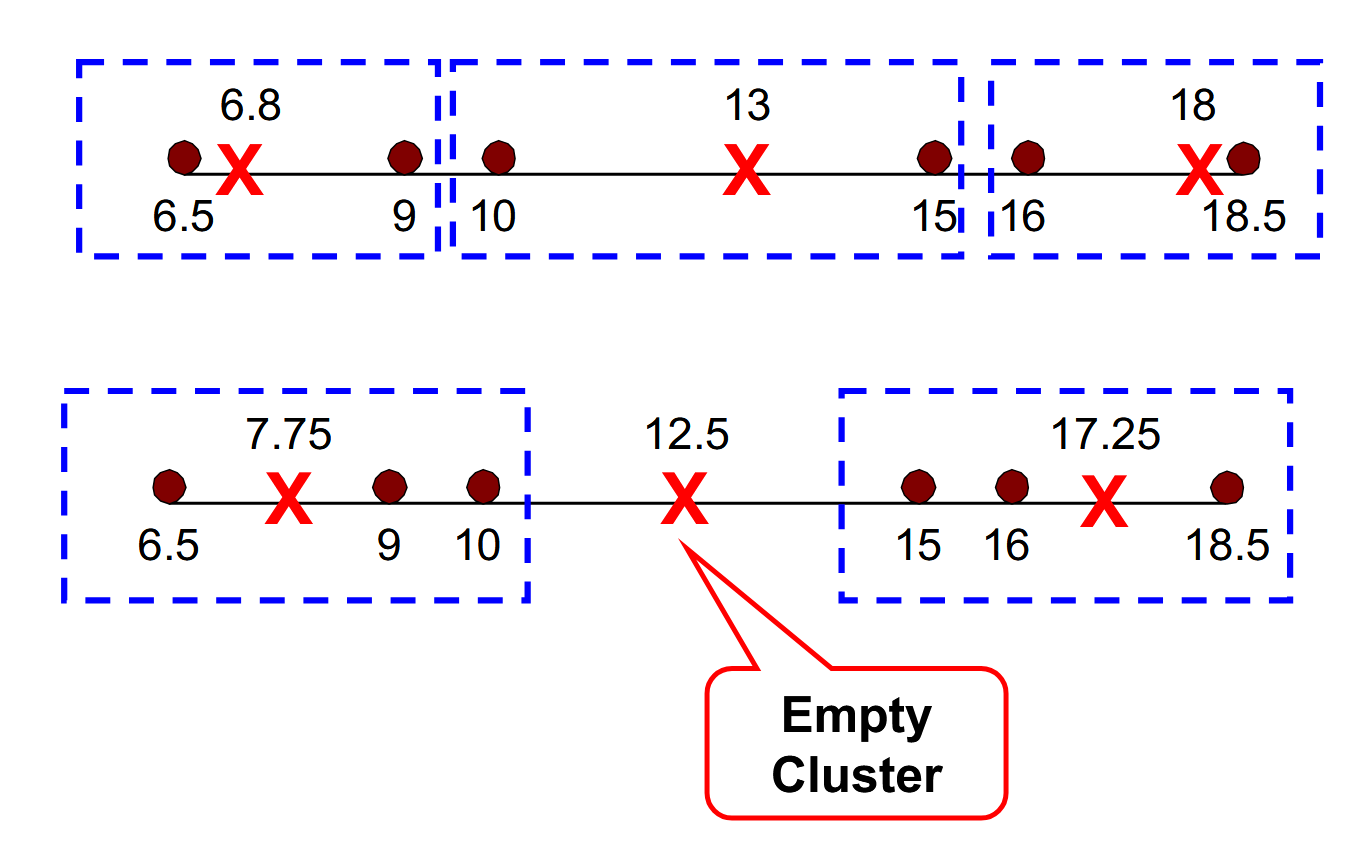
\includegraphics{images/04/kempty.png}
		\caption{K-Means with Empty Clusters}
		\label{fig:04/kempty}
	\end{figure}
\end{paracol}

\subsection{Workflow}
\begin{enumerate}
	\item Data Preprocessing
	      \begin{itemize}
		      \item Handle missing values
		      \item Normalize/standardize data
	      \end{itemize}
	\item Choose the number of clusters $K$
	\item Post processing and validation
	      \begin{itemize}
		      \item Eliminate small clusters that may represent outliers
		      \item Split ‘loose’ clusters, i.e., clusters with relatively high
		            SSE
		      \item Merge clusters that are ‘close’ and that have relatively
		            low SSE
		      \item Can use these steps during the clustering process\\
		            \texttt{ISODATA}
	      \end{itemize}
\end{enumerate}

\subsection{Choosing the number of clusters K}
If there are K ``real'' clusters then the chance of selecting
one centroid from each cluster is small, especially if K is large.

A solution is to run K-Means multiple times with different initial centroids and choose the best result, but probability of getting a good result is still small.

A different approach is to use \textbf{hierarchical clustering} to determine initial centroids for K-Means.

Another option is to \textbf{incrementally} update centroids as points are assigned to clusters, instead of waiting until all points are assigned.
This is more expensive and introduces order dependence.
\nl

We can define a goodness measure of a cluster $c$ (hence of the set of Clusters $C$) as the SSE from the cluster centroid:
\begin{align}
	SSE_C(c,s) &= \sum_{i=1}^{n} (d_i, s_c)^2\\
	G(C,s) &= \sum_{c \in C} SSE_C(c,s)
\end{align}
where $s_c$ is the centroid of cluster $c$, $d_i$ is a point in cluster $c$, and $C$ is the set of clusters.

Re-assignment of points to clusters and re-computation of centroids is guaranteed to \textit{not increase} (or \textit{monotonically decreases}) $G(C,s)$, hence K-Means converges to a local minimum.

At any step we have some value for G(C,s),
\begin{enumerate}
	\item Fix $s$, optimize $C$ $\rightarrow$ Assignment step: assign $d_i$ to the closest centroid $\Rightarrow G(C',s) \leq G(C,s)$
	\item Fix $C'$, optimize $s$ $\rightarrow$ Update step: recompute centroids $\Rightarrow G(C',s') \leq G(C',s) \leq G(C,s)$
\end{enumerate}
In this way the new cost results smaller than the original one, leading to convergence to a local minimum.